\subsection{Ethernet Switch}
The Ethernet switch bridges communication between 3 crucial components: the host PC, the robot controller, and the PLC. The Ethernet switch is located within the control cabinet and insures consistent and instantaneous communication over the network.
\begin{figure}[h!]
	\centering
 	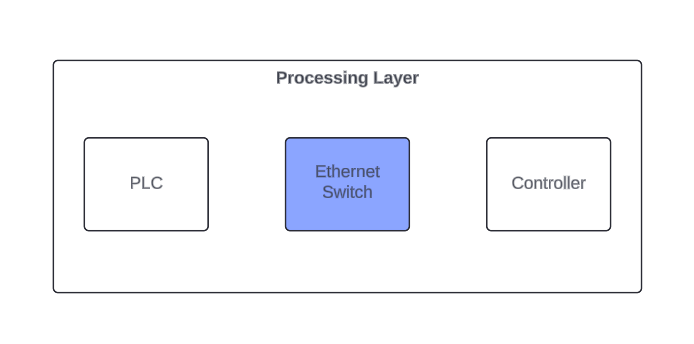
\includegraphics[width=0.60\textwidth]{images/Processing_Ethernet.png}
 \caption{Ethernet subsystem}
\end{figure}

\subsubsection{Assumptions}
A stable Ethernet connection is assumed for consistent data transfer. The components are configured to be on the same sub-network to communicate. Additionally, the robot controller and PLC must be configured with Mitsubishi's CC-Link IE Field Network to ensure signal transfer.
\subsubsection{Responsibilities}
The Ethernet switch is responsible for routing and forwarding data packets between the robot controller, PLC, and other networked devices. The switch must be consistent to ensure precision and fast transmission. Without the Ethernet switch, the robotic work cell cannot function properly and errors will arise from a lack of communication.

\subsubsection{Subsystem Interfaces}

\begin {table}[H]
\caption {Subsystem interfaces} 
\begin{center}
    \begin{tabular}{ | p{1cm} | p{6cm} | p{4cm} | p{5cm} |}
    \hline
    ID & Description & Inputs & Outputs \\ \hline
    \#04 & Data input from PC & \pbox{4cm}{CAT6 Ethernet Cable} & \pbox{5cm}{CC-Link processed packets}  \\ \hline
    \#05 & Data input from PLC & \pbox{4cm}{CAT6 Ethernet Cable} & \pbox{5cm}{CC-Link processed packets}  \\ \hline
    \#06 & Data input from CR-800 Controller & \pbox{4cm}{CAT6 Ethernet Cable} & \pbox{5cm}{CC-Link processed packets}  \\ \hline

    \end{tabular}
\end{center}
\end{table}

\subsection{Controller}
Controllers are designed to seamlessly integrate with robots. These sophisticated devices serve as the brain of robots, governing their actions and enabling precise control.
%The Raspberry Pi serves as an integral component of the processing unit within the robot system. It fulfills the role of an edge computing device, responsible for initial data processing and interfacing between the sensors and the host PC. Specifically, the Raspberry Pi is responsible for collecting data from a variety of sensors, including those for QR code scanning and other environmental monitoring.
\begin{figure}[h!]
	\centering
 	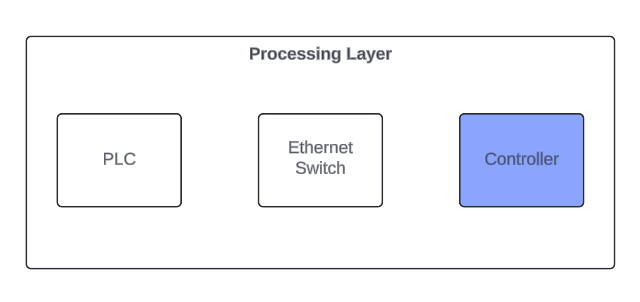
\includegraphics[width=0.60\textwidth]{images/Processsing_controller.png}
 \caption{Controller subsytem}
\end{figure}

\subsubsection{Assumptions}
The primary role of a robot controller is to receive instructions from a PLC and external sensors.

    
\subsubsection{Responsibilities}
Responsibilities of controller is to precisely manipulate the robot's joints according to a specific sequence or pattern. In addition, it also receives signals from E-stops which halts the robot functionality.

\subsubsection{Subsystem Interfaces}

\begin {table}[H]
\caption {Subsystem interfaces} 
\begin{center}
    \begin{tabular}{ | p{1cm} | p{6cm} | p{4cm} | p{5cm} |}
    \hline
    ID & Description & Inputs & Outputs \\ \hline
    \#07 & Controller & \pbox{4cm}{signals} & \pbox{5cm}{movement of joints}  \\ \hline
    \#08 & Controller & \pbox{4cm}{Emergency stops} & \pbox{5cm}{Halting the robot movement}  \\ \hline
    \end{tabular}
\end{center}
\end{table}


